\chapter{State-of-the-Art}\label{chap:sota}
\section{Animation of Single Characters}
\subsection{Sketch-Based Animation}
Guay et al. originally proposed the line of action as a posing tool. In ``The Line of Action: an Intuitive Interface for Expressive Character Posing'' (\citep{guay2013line}), there were several contributions: adapting the line of action (LOA) in the form of a new notation to posing 3D characters, solving the LOA problem as an optimization problem, and validating this technique by having users recreate poses from images. 

From this paper came a prototype, in which a user can draw a line in the shape they want a set of bones to take. They take advantage of the limited amount of kinematic chains called \index{body line@ body line, body lines}\textbf{body lines}. There are said to be only 10 possible body lines, when constrained to be maximal -- meaning that they must end at an extremity -- connected, and linear -- meaning the body line must be a straight line through the tree with no other nodes connected. Even with this constraint, adding more characters allows more combinations of bones.

\begin{figure}[!h]
\centering
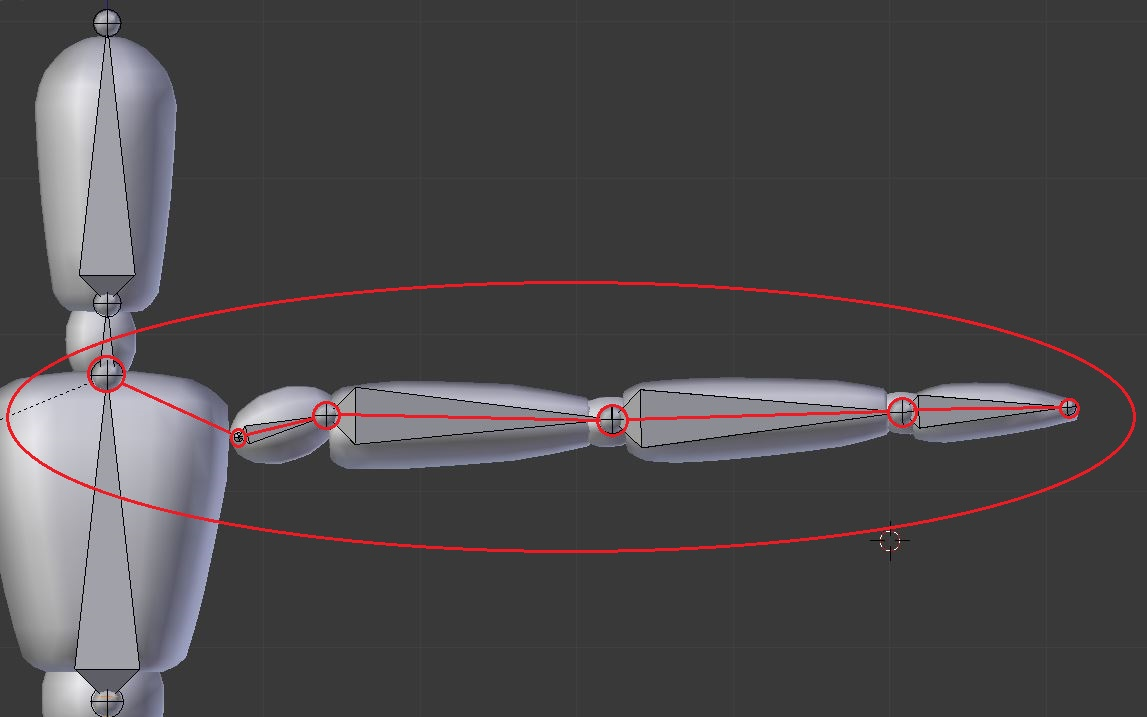
\includegraphics[scale=0.4]{img/shoulder}
\caption{An example of a connected and linear selected body line.}
\end{figure}

Engineers in the IMAGINE team at Inria have implemented the solution of the LOA problem within software called Rumba. In this software, the user draws a selection line to select one of the 10 kinematic chains. Then the user draws a second target posing line to move the body line to a new shape and position. Their system works extremely well for a single humanoid character, and even multiple humanoid characters which are strictly separate from each other.

\begin{figure}[!h]
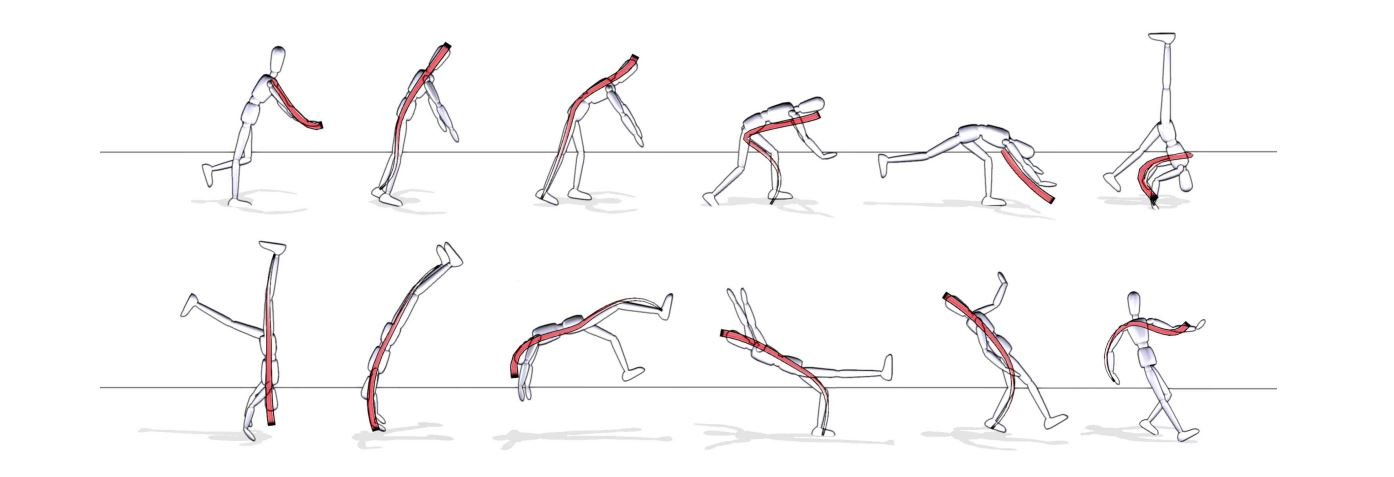
\includegraphics[scale=0.4]{img/baseline}
\caption{One character's keyframes using the line of action technique from \citep{guay2013line}.}
\end{figure}

\ignore{
Noticing that lines of actions can visually suggest the potential energy of a motion, Guay et al. wrote ``Adding dynamics to sketch-based character animations.'' (\citep{guay2015adding}) They turn the line of action into a one with physical properties. They derive an elastic model for the motion of the line.

\begin{figure}[!h]
\centering
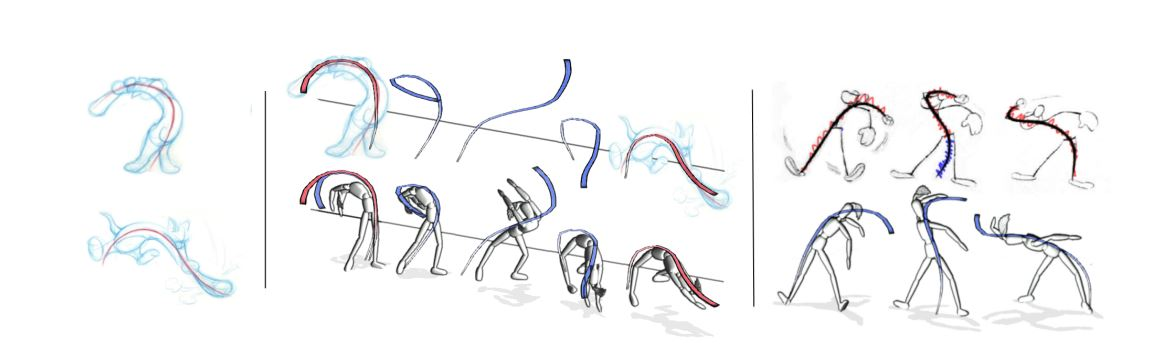
\includegraphics[scale=0.4]{img/dynamics}
\caption{The dynamic line of action. \citep{guay2015adding}.}
\end{figure}
}

In \citep{guay2015space}, Guay et al. continued their work on the line of action to create a technique for animation called space-time sketching, in which a user can draw a line in the path they want a model to take and it will be animated accordingly. As the character follows the path, its model bends and changes shape in a physically realistic way. Their system currently supports creating different movements with the path such as bouncing, rolling, and twisting.

The biggest improvement from their first paper to this one in regards to this work is the linear time algorithm for matching a 3D skeleton to a drawn LOA. This more numerically stable approach to matching the character to the line makes for faster results than the formerly used minimization problem.

\begin{figure}[!h]
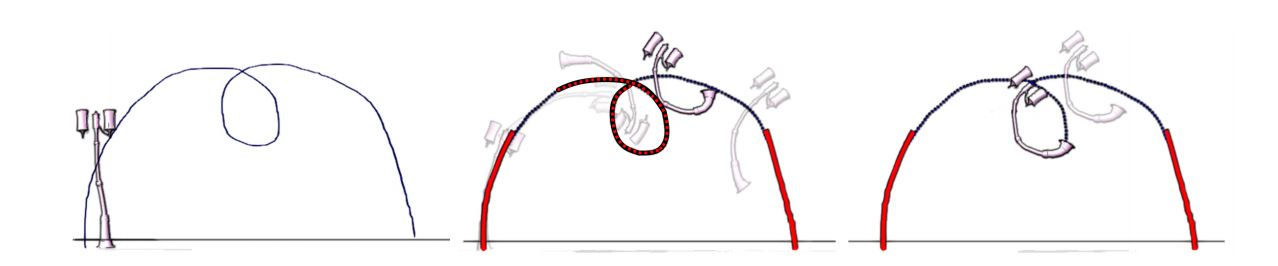
\includegraphics[scale=0.4]{img/rolling}
\caption{A lamp post model rolling. \citep{guay2015space}.}
\end{figure}

Similarly, \citep{mahmudi2016artist} and \citep{stelzleni2015sketch} respectively describe \'Ecole Polytechnique F\'ed\'erale de Lausanne's and Pixar's use of sketching to pose characters. In \citep{mahmudi2016artist}, slight improvements in fitting the body line to the LOA, which is still linear. They also provide automatic body line selection based on the joint the user selects plus the direction of their sketching. There is no mention in either paper about handling the interactions of characters. 

\begin{figure}[!h]
\centering
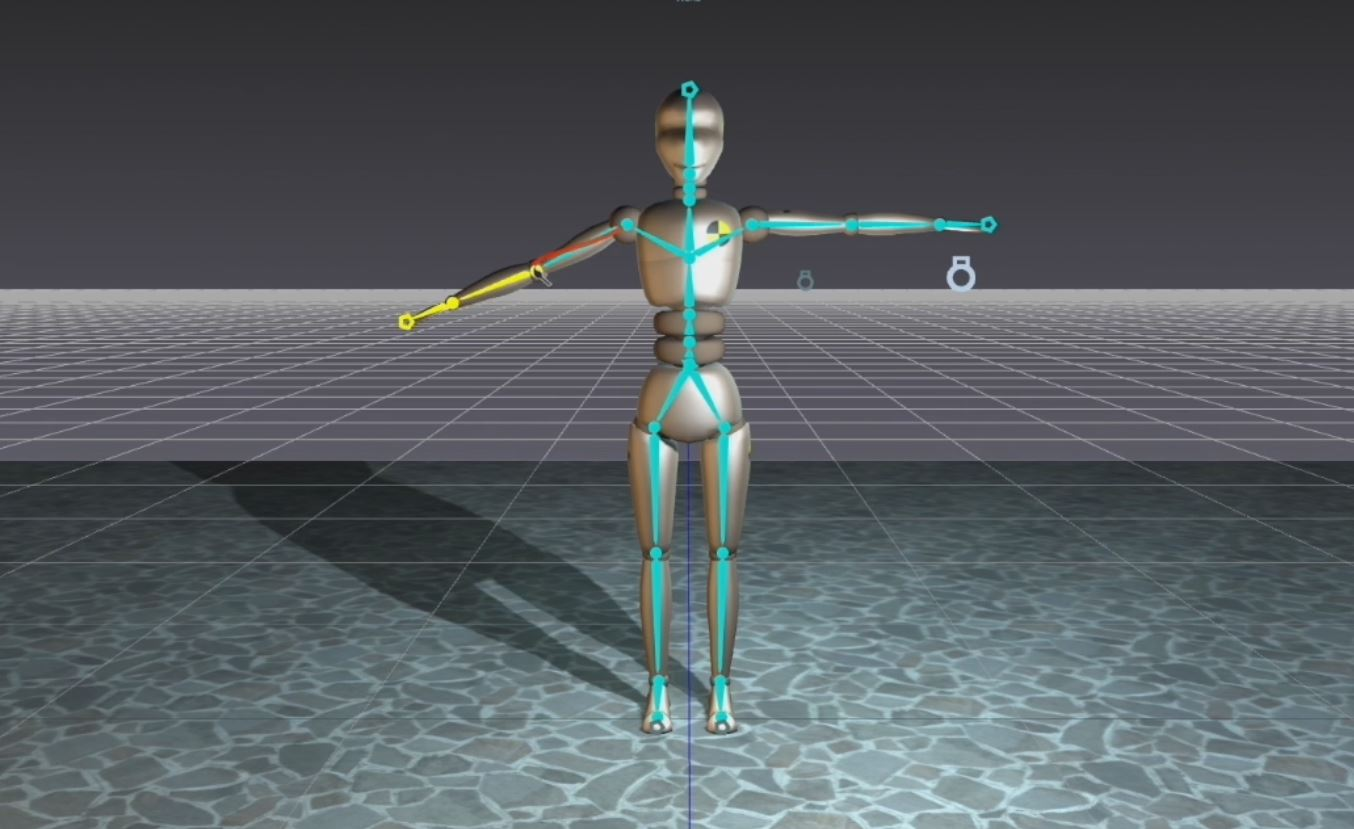
\includegraphics[scale=0.3]{img/epfl}
\caption{ \citep{mahmudi2016artist}'s sketch-based posing system. As the user draws starting from the shoulder, the rest of the arm is highlighted as the automatically selected body line.}
\end{figure}

``SketchiMo: Sketch-based Motion Editing for Articulated Characters'' (\citep{choi2016sketchimo}) is yet another paper which takes advantage of the convenience and ease of a sketch-based interface. This time,  Choi et al. take an already saved animation and visualize the motion through time as different curves. The purpose is to allow the user to edit an existing animation, not create one. Additionally, their demo and paper focus on the animation of a single character.

\begin{figure}[!h]
\centering
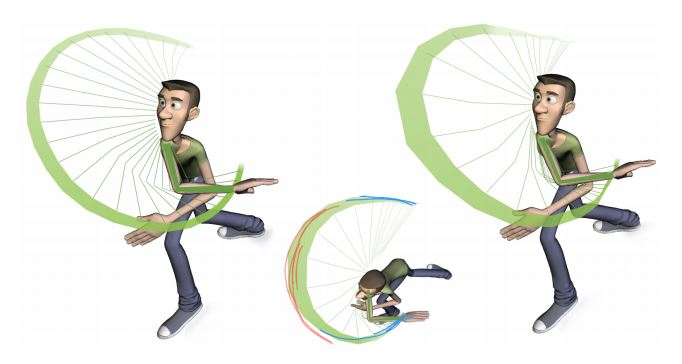
\includegraphics[scale=0.5]{img/sketchimo}
\caption{Animation re-timing in \citep{choi2016sketchimo}.}
\end{figure}

\subsection{Articulated Characters}
Chris Hecker's ``My Adventures with Inverse Kinematics'' (\citep{hecker2002my}) compares and contrasts different inverse kinematics algorithms to animate a character climbing a rock wall. Articulated character animation is challenging due to the combination of contraints that limits the viability of a pose. In his work with the \index{cyclic coordinate descent@cyclic coordinate descent, CCD} cyclic coordinate descent (CCD) algorithm, whose calculations must start at a fixed root, Hecker decides to dynamically change the root of the human's kinematic tree based on what makes the most sense. The idea of root changing can be particularly helpful in the case of combining kinematic trees, though this talk only deals with one character.

Articulated characters are complicated to animate. To this end, generating animation is sometimes easier than doing it by setting a character's pose over and over. Many researchers tackle the problems that come with using motion capture data instead of manually keyframing. The following articles explore generating animation and reusing animation.

In ``Motion Graphs'' (\citep{kovar2002motion}) and ``Style-Based Inverse Kinematics'' (\citep{grochow2004style}), the authors give two different generative methods used to build animations from motion capture sequences. \citep{kovar2002motion} shows how to construct a graph encoding the different orderings of clips that could possibly make up a realistic animation, while \citep{grochow2004style} makes use of a generative machine learning model to easily apply a likely and reasonable style to an existing clip.

``Using an intermediate skeleton and inverse kinematics for motion retargeting'' (\citep{monzani2000using}) is an important paper since it touches upon the idea of changing a skeleton, albeit for retargeting motion rather than creating. This paper describes the usage of an intermediate skeleton when retargeting aninimation from one character hierarchy to another.

\section{Animation of Multiple Characters}
Interactions of multiple characters has never been explored in sketch-based animation, but interactions in general have proved to be another difficult research problem. The following papers show the difficulties of animating by hand, since they all heavily rely on motion capture to provide the animations.

\citep{shum2007simulating} focuses on fighting as an example of close character interactions. This paper also uses motion capture data of single characters to create action-level motion graphs to generate realistic and competitive interactions.
  
\citep{ho2014multi} and \citep{zhao2017character} aim to describe the dynamic spatial relations between characters and also between characters and objects. They both propose an interaction surface or mesh which is multi-structured. \citep{ho2014multi} uses this surface to adapt motion capture data to accomodate new contraints and different character sizes. \citep{zhao2017character} uses the interaction bisector surace, seen in \autoref{fig:ibs}, to retrieve similar motions from a database given a 3D animated clip.

\begin{figure}[!h]
\centering
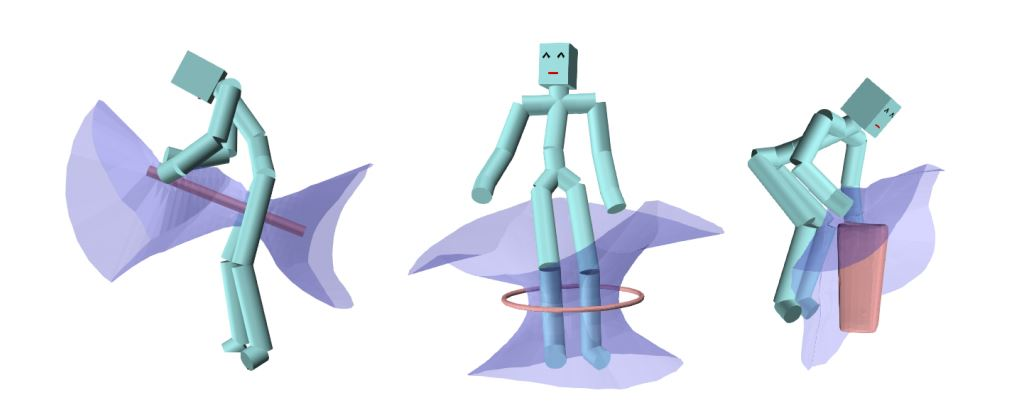
\includegraphics[scale=0.5]{img/ibs}
\label{fig:ibs}
\caption{The interaction bisector surface.}
\end{figure}


\section{Animation of Dancers}
\subsection{Dance Notation}
Valerie Sutton is a choreographer responsible for inventing Sutton Dance Writing, introduced in \citep{sutton1979sutton}. Sutton notation remains the closest inspiration for the line of action. A human dancer is represented as a stick figure drawing, putting emphasis on the expressive shape of poses that are prevalent in dance.

\begin{figure}[!h]
\centering
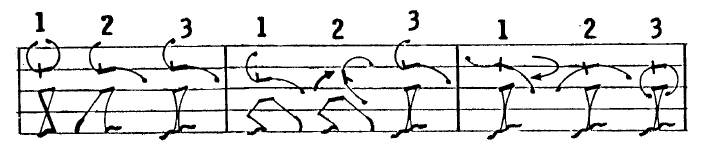
\includegraphics[scale=0.5]{img/sutton}
\caption{An example of Valerie Sutton's Dancewriting.}
\end{figure}

Benesh Movement Notation (introduced in \citep{causley1980introduction}) is analagous to Sutton notation, but for motions instead of poses. This tells a dancer how to transition from one poses to another, exactly like interpolation between keyframes. This notation is complex and not intuitive; it requires a certain amount of study before one can learn to write a dance in this form.

\begin{figure}[!h]
\centering
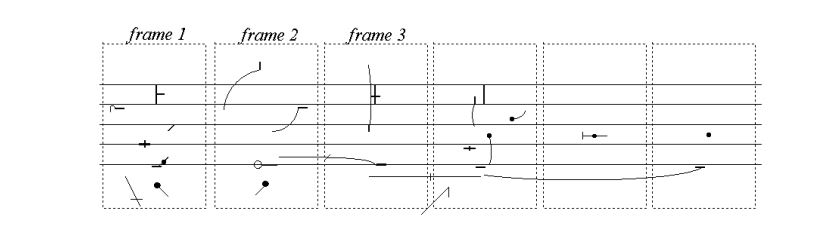
\includegraphics[scale=0.5]{img/benesh}
\caption{An example of Benesh Movement Notation.}
\end{figure}

Labanotation is another way of recording human movement. Rudolph Laban invented it with the purpose of annotating dances. Rather than use figures though, Labanotation uses more abstract notions to describe properties of a movement. The Dance Notation Bureau has documented dances using this more precise and technical method, though it is arguably not ideal for artists to quickly write a dance.

\begin{figure}[!h]
\centering
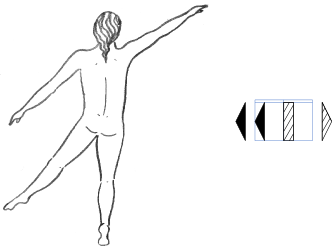
\includegraphics[scale=0.5]{img/over-labanotation}
\caption{An example of Labanotation.}
\end{figure}

\subsection{Dance in Animation}
There is a strong interest in portraying dance in animation, which can be seen in many examples of films over the years:

\begin{figure}[h!]
	\centering
        \begin{subfigure}[b!]{0.3\textwidth}
        	\centering
                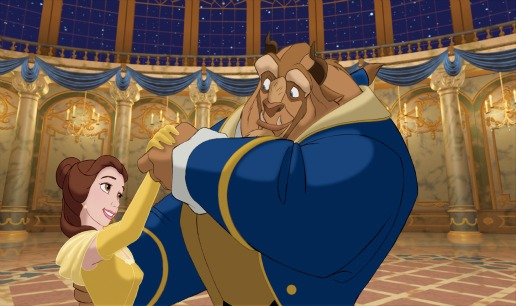
\includegraphics[width=\linewidth]{img/belleetlabete}
                \label{fig:belle}
                \caption{A capture from \textit{Beauty and the Beast.}}
        \end{subfigure}
        \quad
        \begin{subfigure}[b!]{0.3\textwidth}
        	\centering
                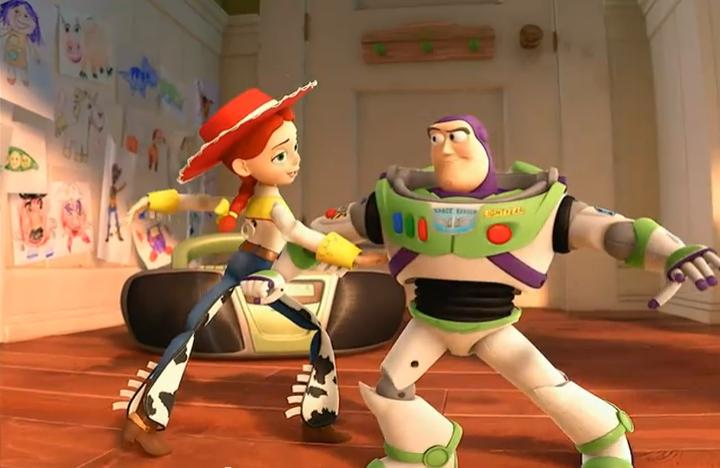
\includegraphics[width=\linewidth]{img/buzz-and-jessie}
                \label{fig:toystory}
                \caption{Buzz LightYear and Jessie dance.}
        \end{subfigure}%
        \quad
        \begin{subfigure}[b!]{0.3\textwidth}
        	\centering
                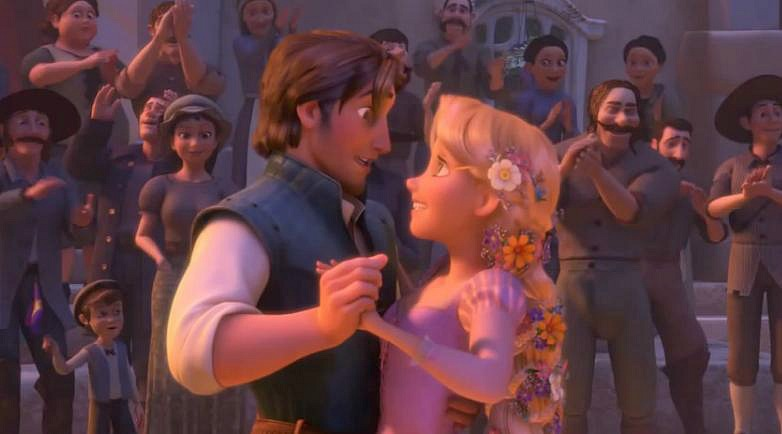
\includegraphics[width=\linewidth]{img/tangled}
                \label{fig:tangled}
                \caption{A scene from \textit{Tangled.}}
        \end{subfigure}%
        \caption{Images from \protect\citeonline{dancemovies}.}
	\label{fig:danceinmovies}
\end{figure}

It has progressed from live action to 2D animation to 3D animation. It is safe to say thqt dance will always be an important part of the human experience and will therefore continue to be represented in art, including film and animation.

So it seems almost obvious that researchers must also be interested in dance in animation. In Gleicher's 1998 paper, \citep{gleicher1998retargetting}, he describes a method of retargetting motion from a motion capture database to 3D articulated characters of different sizes, of which an application is dancing.

\begin{figure}[!h]
\centering
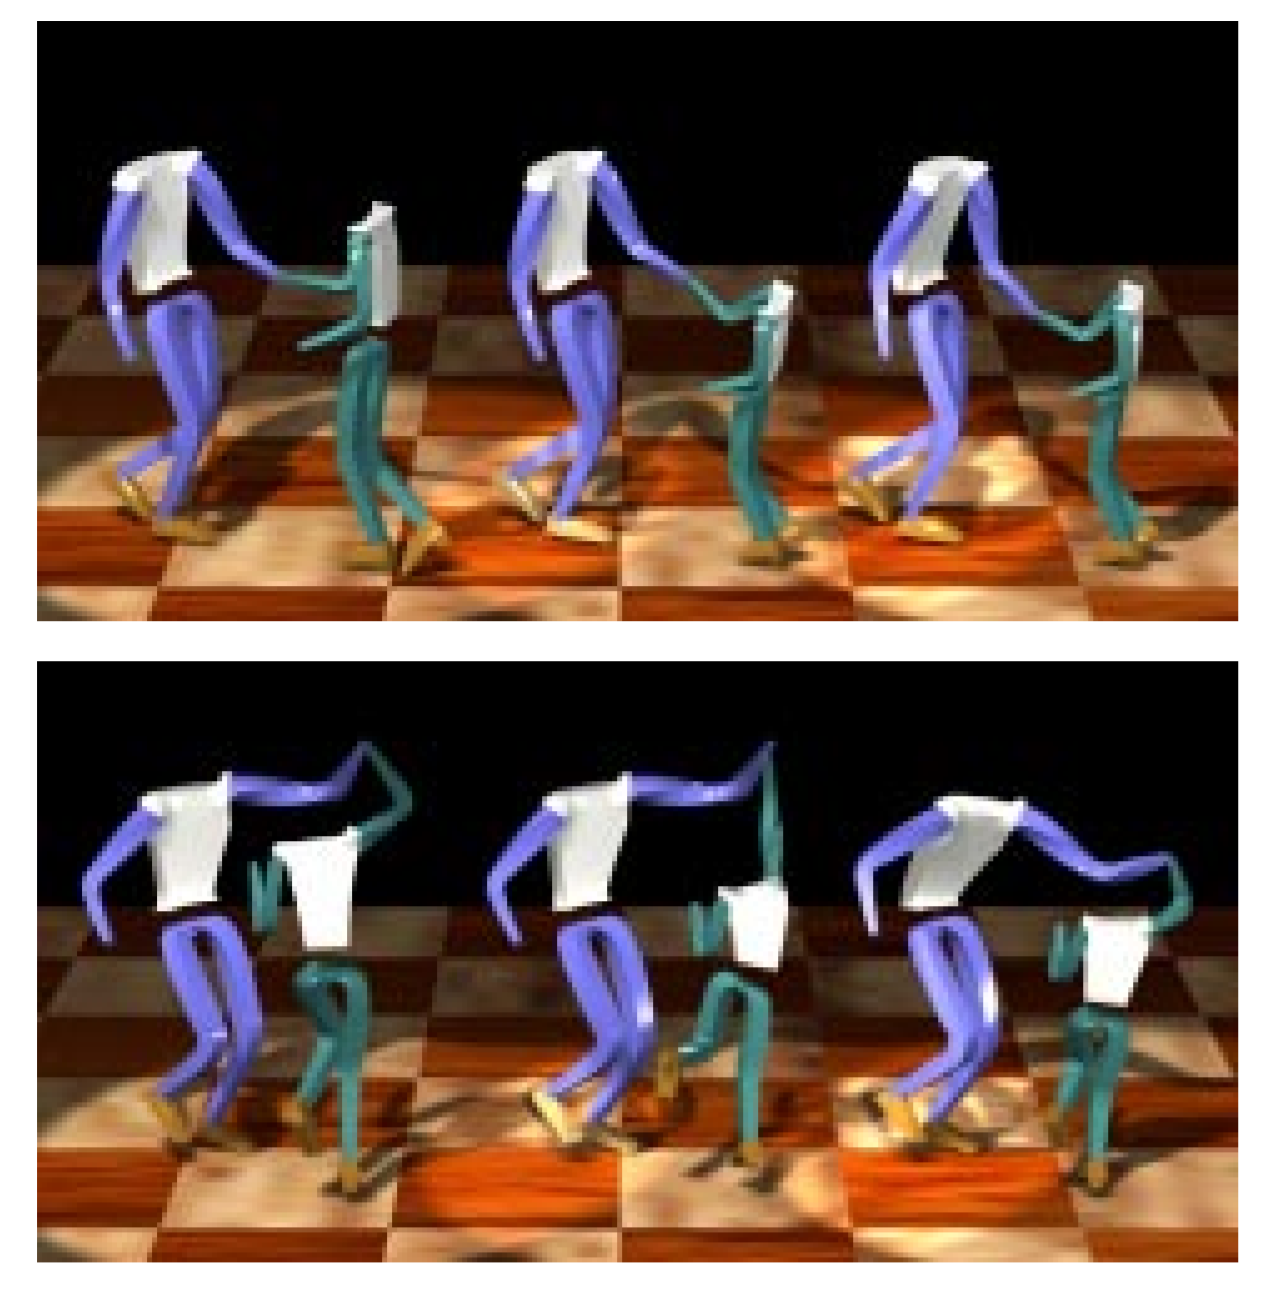
\includegraphics[scale=0.5]{img/retarget}
\caption{Motion retargetting applied to dance from \citep{gleicher1998retargetting}.}
\end{figure}

Based on the 2005 paper \citep{calvert2005applications}, which involves a system for composing and editing dances using Labanotation, Matthews  et al. experimented with procedurally generating dance motion in the paper \citep{matthews2011procedural} using foot motions and basic patterns. \citep{shiratori2006dancing} and \citep{shiratori2006synthesizing} synthesize music and an animation generated from a motion graph built from motion capture data. It attempts to capture the emotional aspects of human dance, which is a shared goal of the line of action.
